\documentclass{article}

% if you need to pass options to natbib, use, e.g.:
%     \PassOptionsToPackage{numbers, compress}{natbib}
% before loading neurips_2019

% ready for submission
\usepackage{neurips_2019}
\usepackage[pdftex]{graphicx}
% to compile a preprint version, e.g., for submission to arXiv, add add the
% [preprint] option:
%     \usepackage[preprint]{neurips_2019}

% to compile a camera-ready version, add the [final] option, e.g.:
     %\usepackage[final]{neurips_2019}

% to avoid loading the natbib package, add option nonatbib:
%     \usepackage[nonatbib]{neurips_2019}

\usepackage[utf8]{inputenc} % allow utf-8 input
\usepackage[T1]{fontenc}    % use 8-bit T1 fonts
\usepackage{hyperref}       % hyperlinks
\usepackage{url}            % simple URL typesetting
\usepackage{booktabs}       % professional-quality tables
\usepackage{amsfonts}       % blackboard math symbols
\usepackage{nicefrac}       % compact symbols for 1/2, etc.
\usepackage{microtype}      % microtypography

\title{Investigating Network Architectures on Canonical 1D Partial Differential Equations}

% The \author macro works with any number of authors. There are two commands
% used to separate the names and addresses of multiple authors: \And and \AND.
%
% Using \And between authors leaves it to LaTeX to determine where to break the
% lines. Using \AND forces a line break at that point. So, if LaTeX puts 3 of 4
% authors names on the first line, and the last on the second line, try using
% \AND instead of \And before the third author name.

\author{%
  Alejandro Francisco Queiruga\thanks{} \\
  Energy Geosciences Division\\
  Lawrence Berkeley National Lab\\
  Berkeley, CA 94609\\
  \texttt{afqueiruga@lbl.gov} \\
}

\begin{document}

\maketitle

\begin{abstract}
  This paper examines the coincidence of neural networks with
  numerical methods for solving spatiotemporal physical problems.
  Two well understood 1D problems are tackled: the heat equation and
  Burgers' equation. Coincidence is shown by demonstrating that a single layer convolutional neural network converges to a traditional finite difference stencil for the
  heat equation. However, disctriminator-based advsererial training, such as those prevelant in
  the hot-topic of generative adverserial networks, does not find the
  expected 3 weights. A compact deep convolutional network is designed
  motivated by flux winding schemes in finite volume methods. 
  % This work performs a thorough empirical analysis of the application
  % of neural networks to solving well understood partial differential
  % equations.
  % Only one spatial dimension is treated, where pentiful analytical solutions can be evaluated to machine precision to provide datasets with no artifacts.
  % Burger's equation and the Korteweg-de Vries equation are treated,
  % which even are challenging to solve numerically due
  % to their nonlinearity and exhibition of shock fronts even in one spatial dimension.
\end{abstract}

\section{Introduction}

Most extremely challanging physical systems are extremely challenging to describe due to unknown underlying physics or intractable complexities with traditional approaches. Analysis of dynamics data through neural networks and deep learning is a hot topic and very promising approach to learn predictive tools, but the properties are not yet well understood. The problem of discovering dynamics can be stated as follows:
\begin{equation}
\textrm{Given data }\, u_i^k=u(x_i,t_k), \,\textrm{find }f\textrm{ such that }\, u^{k+1}=f(u^k)
\end{equation}
This paper seeks to explore the use of neural networks as an $f$ to discover predictive functions on well known equations (for which decent $f$s are already known.)\footnote{This approach is looking for a function that inputs an image returns and image. Another approach is to look for conditional scalar functions with coordinates as inputs, $u^{k+1}(x,y)=f(x,y|u^{k})$; this was not considered. }
Basic one dimensional partial differential equations are always useful to benchmark to any new numerical technique due to well understood properties and known analytical solutions, which can provide as much data as needed without artifacts from synthesis or acquisition.
Multiple standard types of architectures are applied to each of these
canonical equations.
The experiments are designed to take a few minutes of compute time training to replicate with datasets that even fit within a modern cache.
Applying intuition from well understood physics-and-math-up approaches will improve future approaches, providing insights that can hopefully be applied to problems without known physical descriptions but similarities to canonical problems.


Neural networks have rightfully been given a lot of attention to apply to many domains.
The structure of many physical sciences problems is similar to image and speech processing: e.g., PDEs are just grid or graph convolutions once discretized.
Applying generative adverserial networks to perform forecasting and super resolutions

Koopman theory and dynamic mode decomposition are traditional approaches to discovering dynamics.
Instead of searching for nonlinear transforms to find linear operators, but how well can we seek nonlinear operators?
As opposed to fiting to known PDE terms, can we discover neural networks that match known approximations to the operators?  Can neural networks offer us a richer space to find nonlinear operators?


A variety of rich datasets are available for this task, such as the
John Hopkins Turbulence dataset. However, it is wise to give attention
to problems with known solutions when crafting new methods. Towards
this end, this work focuses on verifying methods 1D PDEs, providing
small datasets.



However, how much of this is due to inherent biases? 
Problems in the physical sciences require more than fuzzy-qualities such as probabilistic classification or pretty behavior in the ``eyeball norm'': fine-grained properties such as regression accuracy and numerical stability are important.
It has even been suggested that the structure of CNNs and not the learning stage is the dominating factor to their performance [deep image prior,\cite{ulyanov_deep_2018,zador_critique_2019}. Thus, devising architectures specifically for physical applications 


This paper looks at two well understood 1D time-dependent problems:
the heat equation, $u_{t} = k u_{xx}$, 
and Burgers' equation,  $u_{t} + u_x u = 0$. The heat equation is linear and has a well
known finite difference stencil. Burgers' equation, however, is very
nonlinear and even yields discontinuous solutions, so calling it a PDE
is a stretch. Many schemes for Burgers' equation exist with various
levels of success, and arguably all of these have an {\em ad hoc}
approach to fixing the numerical problems. CITE GUDONOV, WENO
Even this 1D equation is still an open problem where data-driven
approaches can be applied; the work of
\cite{bar-sinai_data-driven_2018} sought to learn high-order
reconstructions of the flux fields from simulated data. (The authors even approached the ``easier''
viscous form of the equation.)

Generative Adverserial Networks (GANs) are very popular now. However,
does a purely adverserial training method give us the correct answer?
This paper checks the methodology on this simplest problem.

% Multiple equations are known to not fit into a PDE context. E.g., burger's equation becomes discontinuous, and ANOTHER EQUATION NEEDS FRACTIONAL DERIVATIVES. The scale of known PDEs may even be intractable in certain contexts, such as attempting to apply Navier-Stokes to the global climate.

Of further interest, how do we predict very far out in the future? If
it is possible to learn a model that predicts $t+\Delta t$, how do we
predict far in the future given only one initial datapoint? Feeding a
model's input into itself is natural---$u^{k+n}=f(f(...f(u^k)$---but
this requires stability on $f$.
NEURAL ODE PAPER ; RESNET delta T paper

% The equations used in the investigation are summarized in Table \ref{tab:pdes}. (Technically, all but one are actually 2D when including time.)
% These include the linear Poisson's equation, an elliptic equation; the heat equation, a parabolic equation; and the wave Equation, a hyperbolic equation: all three have well-understood finite difference stencils. 
% Burgers' equation, a conservative nonlinear equation known for
%   producing sharp fronts,
% The Korteweg-de Vries Equation equation, a conservative nonlinear equation known for
% producing sharp fronts,
% (One could argue that the notion of a PDE even breaks down for Burgers' equation due to the existence of discontinuities: how can finite differences even be applied?)

% \begin{table}
%   \caption{\label{tab:pdes}PDEs under investigation}
%   \begin{tabular}{lll}
%     \hline
%     Name & Equation & Properties\\
%     \hline\hline
%     Poisson Equation & $u_{xx} = f $ & Linear, elliptic, static \\\hline\
%     Heat Equation & $u_{t} = k u_{xx} $ & Linear, parabolic \\\hline
%     Wave Equation & $u_{tt} = c^2 u_{xx} $ & Linear, hyperbolic\\\hline
%     Advection Equation & $u_{t} + a u_x = 0 $ & Linear, hyperbolic\\\hline
%     Burgers' Equation & $u_{t} + u_x u = 0 $ & Nonlinear, shock waves \\\hline
%     Viscous Burgers' Equation & $u_{t} + u_x u = \nu u_{xx} $ & Nonlinear, general analytical solution \\\hline
%     Korteweg-de Vries Equation & $\partial_t u + 6 u \partial_x u + \partial_{xxx}u = 0$ & Shallow Waves \\\hline
%   \end{tabular}
% \end{table}

Using analytical solutions, two datasets are created for each equation
including 10 trajectories from different initial conditions. These are evaluated on a grid of 41 points in $x$ and 100
snapshots in $t$. Six trajectories are used for training, two are used
for testing, and two are used for validation by self recursion on the
initial condition. % VERIFY THIS
The datasets were created using Sympy and are 1.6MB in total. The
entire study is implemented in PyTorch. The experiments presented run in a few minutes each using a GPU instance. The source code and datasets can be found at https://github.com/{\em hidden for blind review.}



\section{Models For Spatiotemporal Systems}

\begin{figure}
  \centering
  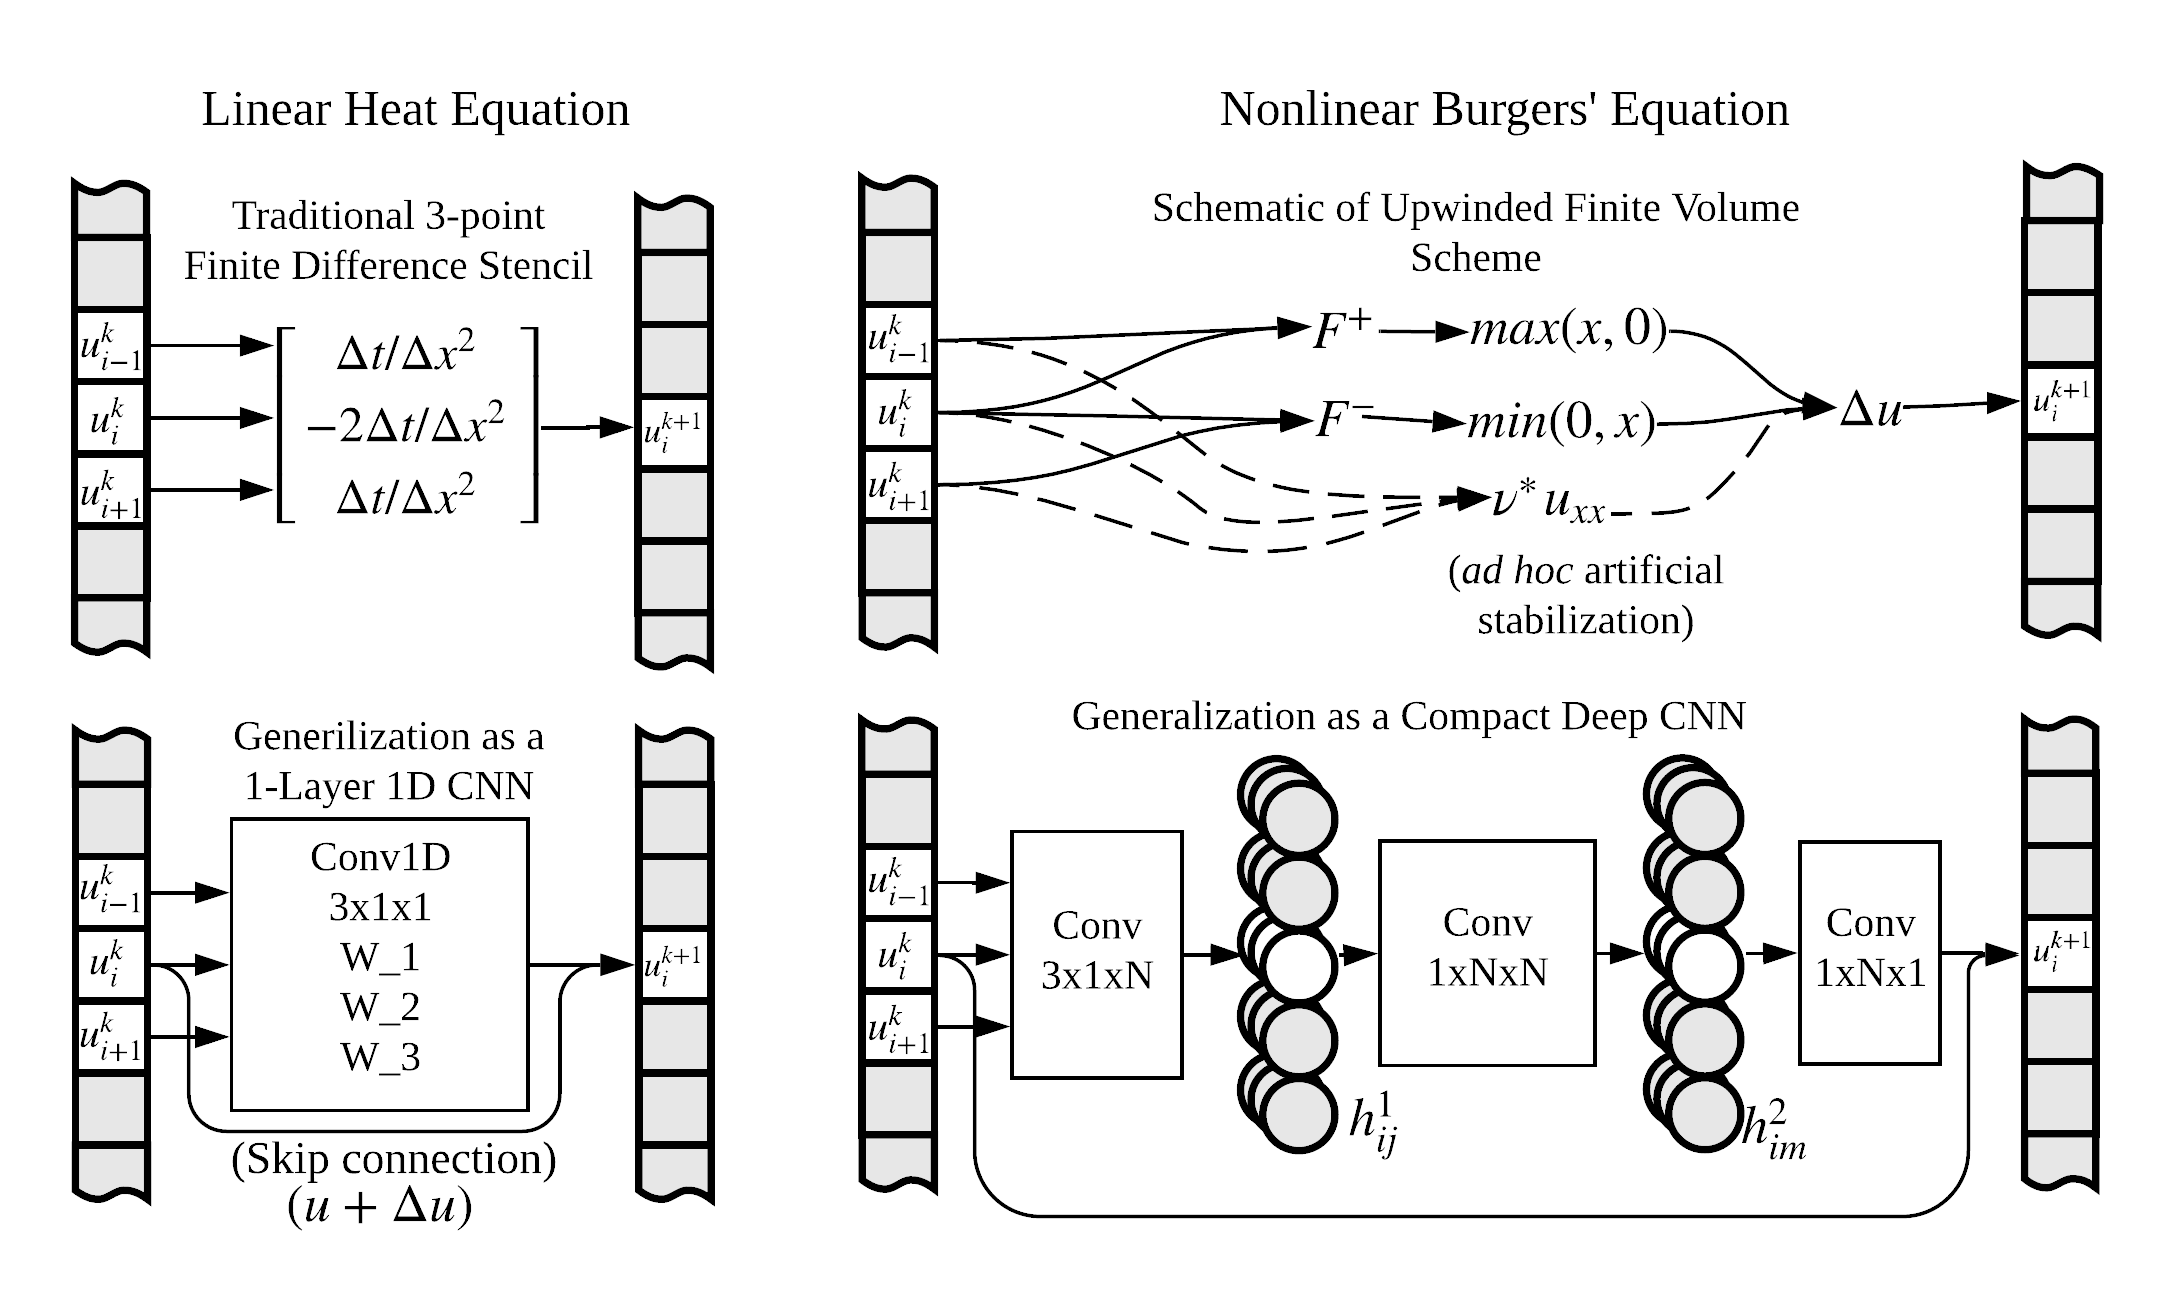
\includegraphics[width=5in]{CNN_FDM.png}  
  \caption{\label{fig:cnn_fdm}Coincidence of CNNs with existing finite difference
    schemes. On the left, a one-layer CNN is the same as the traditional 3-point finite difference
    stencil. It is demonstrated that the 3 weights converge to the
    expected parameters. On the left, a finite volume scheme for
    Burgers' equation requires a complex nonlinear flow graph with
    decision trees for winding and additional stabilization terms. A generalized CNN can attempt to
    discover a similar, or even better performing, method. Including the skip connection
    allows the model to be generalized to other timestep sizes, and
    might improve recurrent training.}
\end{figure}

As illustrated in Figure \ref{fig:cnn_fdm}, the numerical schemes
developed over the years can viewed as a fringe case of a certain CNN
architecture. The finite difference method derives using stencils from
Taylor expansions that turn into update rules for the next time step:
\begin{equation}
  u^{k+1}_{i} = u^k_{i}+\mathtt{stencil}\left( u^k_{i-1}, u^k_{i},u^{k}_{i+1}; \Delta x, \Delta t\right)
\end{equation}
The classical stencil for the heat equation is
$u^{k+1}\\approx u^k+(k\Delta t)(\Delta x^2) \left(u_{i-1} - 2 u_{i} +
  u_{i+1}\right)$.
This architecture corresponds to a fringe case neural network: a
3-weight 1D convolutional neural network (CNN) with no bias and no
activation function. This interpretation
generalizes to wider stencils and more dimensions, but this is the
simplest possible problem.
Verifying that these coefficients can be derived by the optimization
algorithm is a good first step: below, it is shown that the standard
ADAM optimizer will discover this stencil.

% Question: Do we want to learn $u^{k+1}$ or $\Delta u^{k+1}$?
% The paper THAT ONE ABOUT RESNET showed a technique to describe
% residual networks as iterative time stepping methods to improve
% training.
% The effect on training is tried by adding a skip connection to all of the models--- $f(x)=\mathbf{net}(x)+x$---so that $\mathbf{net}$ learns the rate. This would further allow changing $\Delta t$ or generalize to other time integration schemes, but this was not explored.

The modle input is an $N_x$ array. Boundary conditions are neglected;
the first and last entry of the array are set to the analytical
solution in the dataset when performming recurrent prediction.

% performing recurrent prediction, the values at the edges of the domain are set to
% the known analytical solution to ensure that improper treatment of the
% boundaries do not contaminate the results, yielding pure Dirrichlet
% boundary conditions every. The boundary domain is extended to the
% sencil width. The model output is thus padded by the correct amount of 0s to make the output an $N_x$ array.


% \begin{table}
%   \caption{\label{tab:network}Network Architectures Used}
%   \begin{tabular}{llc}
%     \toprule
%     Name & Description & No. of Parameters \\
%     \midrule
%     PureStencil & Conv(1,1,3,bias=False) & 3 \\
%     PureLinear & Linear($N_x$,$N_x-2$,bias=False) & 1,599 \\
%     FCMLP & & \\
%     Linear Conv & & 3 \\
%     Pure-ConvMLP & &  \\
%     Autoencoder & & \\
%     U-Net & &  \\
%     Recurrent & & \\
%     \midrule
%     Discriminator & Conv(3,1),Pool(3,1), AdptPool(1), Sigmoid & \\
%     \bottomrule
%   \end{tabular}
% \end{table}


Compact means that only the first layer has width. Every successive
layer is one-wide, and no pooling appears. This allows the network to
be applied to a domain of any size, and enforces the locality
constraint of the physics.




\section{Heat Equation}

The time frequency of snapshots used for training will affect training.
Recall the Courant–Friedrichs–Lewy (CFL) condition dictating the ratio
of spatial and temporal discretization spacings to ensure stability
for explicit schemes: for the heat equation, $\delta t / \delta x < C$ or $\delta t / \delta
x^2<C$ for some positive $C$ \cite{leveque_finite_2007}.

% The standard metric is the L2 loss function:
% \begin{equation}
% L\left(u^k,u^{k+1}\right) = \left\| u^{k+1}_i-f(u^k) \right\|_2^2.
% \end{equation}

% % Multiple input steps effects the network architecture:
% \begin{equation}
% L\left(\left\{u^k,u^{k-1}...u^{k-P}\right\},u^{k+1}\right) = \left| u^{k+1}_i-f(u^k,...u^{k-P}) \right|
% \end{equation}


A combination of standard training using the mean squared error and
adverserial training with a discriminator is considered. A conditional discriminator $D(y|x)$ is optimized which learns, given $x$, determine if $y$ is the datum or the model prediction. For these problems, no stochastic effects are included, and the model and evaluation of the discrimanor are perfectly deterministic. Thus, the inclusion of discriminatoris essentially {\em learning a loss function}, replacing the mean-squared-error loss with potentially something better: 
\begin{equation}
L\left(u^k,u^{k+1}\right) = \lambda_1 \left\| u^{k+1}-f(u^k)
\right\|_2^2 + \lambda_2\left(1 - D\left(f(u^k)|u^k\right) + D\left(u^{k+1}|u^k\right)\right)/2
\end{equation}
The cost function to minimize at each step is
$N_{batch}^{-1}\sum_{x,y\in batch} L(y,x)$. \footnote{Averaging this
  loss function over a batch the same way as the others yields the
  $\mathbb{E}_x[1-D(f(x))]-\mathbb{E}_y[D(y)]$ equation of traditional
  GANs, but using ``expected value'' does not quite apply to a fully
  deterministic model.} The weights $\lambda_1$ and $\lambda_2$ are
just set to $(1,0)$, $(0,1)$, and $(1,1)$. When $\lambda_2\neq 1$, the
discriminator $D$ is trained to maximize the cost function alternating
steps with the model $f$.

% \begin{figure}
%   \centering
%   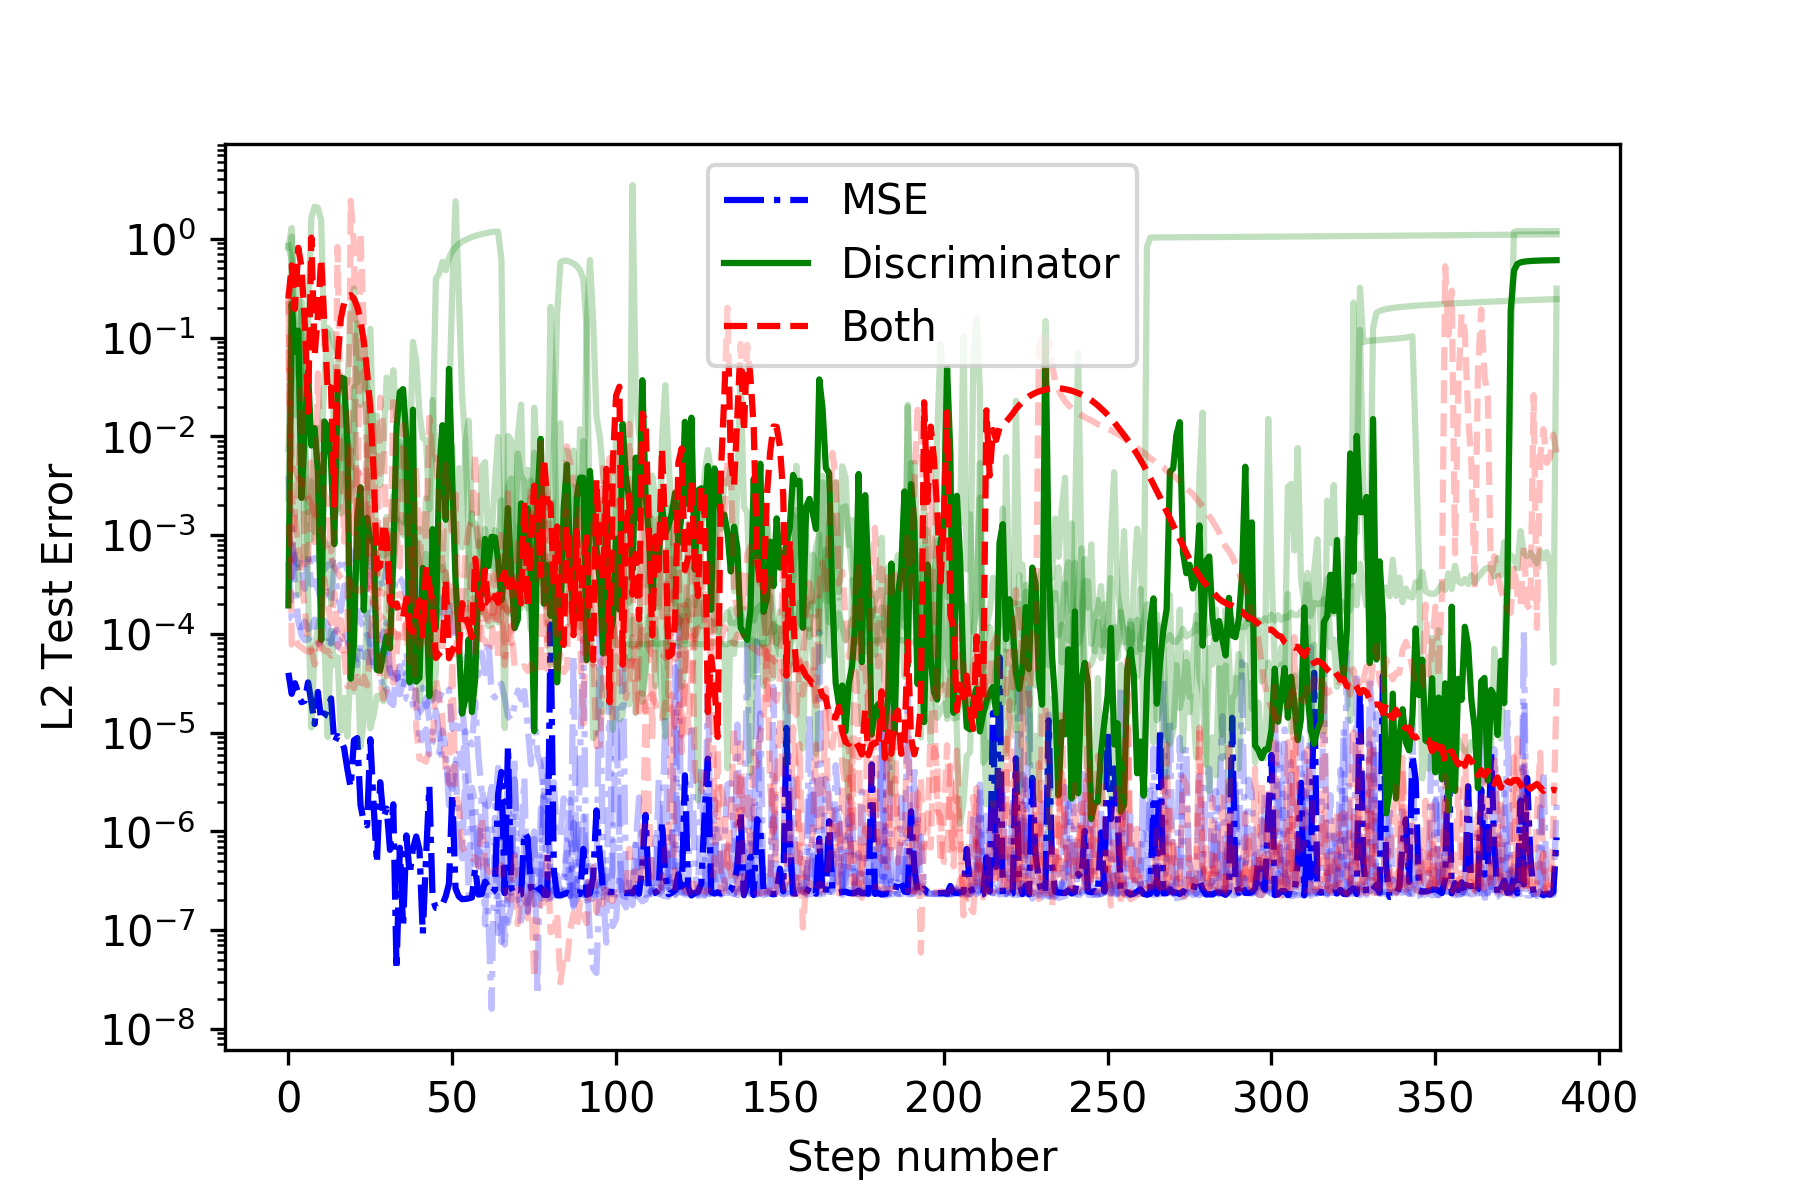
\includegraphics[width=5in]{3pt_L2_loss.png}
%   \caption{Convergence of 3-parameter CNN to the expected stencil
%     using L2 optimization and adversarial
%     training. $10^{-7}$ error is likely the best obtainable in single precision.}
% \end{figure}

\begin{table}
  \caption{\label{tab:conv}The convolutional weights learning by the 3 training
    methods for five randomly initialized runs. The weights are
    divided by $k \Delta t / \Delta x^2$ to normalize to
    $1,-2,1$. Training through a discriminator does not get the
    correct magnitude, but, interestingly, learns the shape of the operator.}
  \centering
  \begin{tabular}{rrr|rrr|rrr}
    \hline
    \multicolumn{3}{c}{MSE} & \multicolumn{3}{c}{Adverserial}  &\multicolumn{3}{c}{Both} \\
\hline
 0.997 & -1.995 & 0.997 & 1.398 & -1.149 & 1.401 & 1.073 & -2.149 & 1.077 \\
 0.997 & -1.995 & 0.998 & 1.058 & -3.196 & 0.956 & 0.994 & -2.000 & 0.995 \\
 0.998 & -1.996 & 0.998 & 1.512 & -0.824 & 1.624 & 0.595 & -1.502 & 0.732 \\
 0.998 & -1.994 & 0.999 & 1.084 & -1.154 & 1.116 & 1.000 & -2.001 & 1.000 \\
 0.998 & -1.995 & 0.998 & 1.392 & -0.558 & 1.394 & 1.000 & -1.999 & 1.000 \\
\hline
\end{tabular}
\end{table}




The first sanity check was to derive the $[1,-2,1]$ stencil from the heat equation dataset with a three-parameter CNN.
Testing the algorithms ADAM, Rprop, and SGD on learning rates of $0.1, 10^{-2}, 10^{-3}, 10^{-4}$, and $10^{-5}$, only ADAM converged to the right answer with $0.1$ and $10^{-2}$. Increasing from single precision to double precision did not change this result. Single precision with a learning rate of $0.1$ was used for the rest of the studies.
This test also verified that the dataset met the CFL condition by
assigning the ``PureStencil'' CNN parameters to the expected answer,
enabling the testing of this barrier.
The architecture of the discriminator is a pooling convolutional
network with three hidden layers and LeakyReLU activation functions, with a total of 51 parameters.
The experiment was repeated 5
times for each loss function to produce the final learned stencils in
Table \ref{tab:conv}.
Using the MSE loss achieves $10^{-7}$ error, which likely the best obtainable in single precision.
Purely adverserial training with a learned discriminator does not learn the same stencil. It appears that the discriminator only learns the ``parabolic'' shape to it, but not the magnitude. Combining the discriminator loss and L2 loss improve training and converges to the correct stencil with correct magnitude.
%When observing the learned values during training, it was observed that the $[1,-2,1]$ ``shape'' of the stencil was trained quickly, but that it took a longer time to optimize to the magnitude.

\section{Burgers' Equation}

The dataset is a series of linear profiles, shock and rarifaction
profiles, and one parabolic profile terminated before the
shock. (These were the only analytical solutions the {\em author(s)}
could find.) The CFL equation for this equation is $\Delta t < C \Delta
x / \max lu|$. 
The compact deep CNN architecture has the following hyperparameters: the number of
features in the hidden layers $n$,the total depth of the network $d$,
and the activation function, $\sigma$.
Conv(1,$n$,3), $\sigma$,Conv($n$,$n$,1)... $d-1$ times... $\sigma$,
Conv($n$,1,1)
The following activation functions were included: ReLU, LeakyReLU, Tanh, CELU, Sigmoid.
The width of the first convolution, 3, was not varied, but could be in
the future.

\begin{figure}
  \centering
  \includegraphics[width=5in]{burgers_loss.png}
  \caption{Convergence of the compact networks for burgers' equation.}
\end{figure}


Learning a discriminator did not have a positive effect on the
results for this problem; searching for a discriminator may be
beneficial. To improve training for the recurrent predicition task,
multiple steps can be included in the training:
\begin{eqnarray}
L\left(u^k,\left\{u^{k+1},u^{k+2}...\right\}\right) =  \left\| u^{k+1}-f(u^k) \right\| + \lambda_1  \left\| u^{k+2}-f \circ f(u^k) \right\| \nonumber \\+ \lambda_2  \left\| u^{k+3}-f \circ f \circ f(u^k) \right\| + ...
\end{eqnarray}
where $\lambda_i$ are weighting coefficients.


\section{Conclusion}
\label{sec:conclusion}

We show that a fringe case of CNN architecture corresponds to a standard finite difference stencil, and converges to the expected coefficients using popular optimizers for NNs on both L2 loss and a learned loss function through adversial training.
Deep CNNs were successfully derived for solving Burgers' equation accurately {\em and } stably.
These results suggest caution to using a purely GAN-type training for physics problems where accuracy is important. The ability to detect the shape of the operator is promising; the {\em author(s)} hypothesize that the discriminator may help with issues such as stability in more complex systems.


Specially designed models that enforce conserved quantities such as
mass and energy, such as the work of YAI et al., are
advantageous, but this requires knowing the quantities {\em a
  priori}. Future seek to design conservative networks that can learn features
that are conserved quantities.


This analogy allows us to interpret the output of our learning algorithms, and guide the design of new architectures for these problems.
This work hopes to provide a simple, well understood benchmark for
proving recently demonstrated ML methods for solving physical systems
developing ML methods for solving physical systems (and remaining as a
tiny unit test to the codebases!)
Studdying the stability properties of recurring these networks applied
to physics problems can extend to stabilizing recurrent networks for
other applications.
By finding this area of overlap between solving PDEs and deep learning, we can seek to bridge the gap and transfer knowledge between the two fields. For example, can methods for L-stable implicit high-order ODE integration be applied to transformer networks?

% \subsection{Margins in \LaTeX{}}

% Most of the margin problems come from figures positioned by hand using
% \verb+\special+ or other commands. We suggest using the command
% \verb+\includegraphics+ from the \verb+graphicx+ package. Always specify the
% figure width as a multiple of the line width as in the example below:
% \begin{verbatim}
%    \usepackage[pdftex]{graphicx} ...
%    \includegraphics[width=0.8\linewidth]{myfile.pdf}
% \end{verbatim}
% See Section 4.4 in the graphics bundle documentation
% (\url{http://mirrors.ctan.org/macros/latex/required/graphics/grfguide.pdf})

% A number of width problems arise when \LaTeX{} cannot properly hyphenate a
% line. Please give LaTeX hyphenation hints using the \verb+\-+ command when
% necessary.

\subsubsection*{Acknowledgments}

{\em Placeholder for blind review.}
% Use unnumbered third level headings for the acknowledgments. All acknowledgments
% go at the end of the paper. Do not include acknowledgments in the anonymized
% submission, only in the final paper.

% \section*{References}

% \medskip

% \small

\bibliographystyle{plainnat}
\bibliography{zotero}

\end{document}
